%%%%%%%%%%%%%%%%%%%%%%%%%%%%%%%%%%%%%%%%%
% Original author:
% Linux and Unix Users Group at Virginia Tech Wiki 
% (https://vtluug.org/wiki/Example_LaTeX_chem_lab_report)
%
% License:
% CC BY-NC-SA 3.0 (http://creativecommons.org/licenses/by-nc-sa/3.0/)
%
%%%%%%%%%%%%%%%%%%%%%%%%%%%%%%%%%%%%%%%%%

%----------------------------------------------------------------------------------------
%	PACKAGES AND DOCUMENT CONFIGURATIONS
%----------------------------------------------------------------------------------------

\documentclass[a4paper,11pt]{article}

\usepackage{graphicx} % Required for the inclusion of images
\usepackage{titling}
\usepackage{upgreek}

\setlength{\droptitle}{-8em}   % This is your set screw

\setlength\parindent{0em} % Removes all indentation from paragraphs

\renewcommand{\labelenumi}{\alph{enumi}.} % Make numbering in the enumerate environment by letter rather than number (e.g. section 6)

\usepackage{times} % Uncomment to use the Times New Roman font

%\usepackage{indentfirst}

\setlength{\parskip}{0.5em plus1pt minus1pt}

%\usepackage{showframe} % for viewing margin frames (debug)

\usepackage{fullpage}

%----------------------------------------------------------------------------------------
%	DOCUMENT INFORMATION
%----------------------------------------------------------------------------------------

\title{SDP Group 8: Final Individual Report} % Title

\author{Blake Hawkins} % Author name

\date{21 April, 2014} % Date of the milestone

\begin{document}

\maketitle % Insert the title, author and date

\begin{center}
\textbf{Mentor:} Katharina Heil, \textbf{Guest Mentor:} Tom Spink % Instructor/supervisor
\\
\textbf{Members:} Blake Hawkins, % Partner names
Lubomir Vikev,
Borislav Ikonomov,
Yordan Stoyanov,
James Linehan,
Lukas Dirzys,
Iain Brown,
Emanuel Martinov,
Robaidh Mackinnon,
Aneesh Ghosh

\end{center}

%----------------------------------------------------------------------------------------
%   SECTION 1 (Introduction)
%----------------------------------------------------------------------------------------

\section{Introduction}

My contributions to our project spanned many topics, each of which will have a section in this report, where I describe them and offer commentary. For brevity, and to meet the two-page limit, many contributions will be left out, and most that were mentioned in previous milestones will be cut short.

%----------------------------------------------------------------------------------------
%	SECTION 2 (Software Design Contributions)
%----------------------------------------------------------------------------------------

\section{Software Design Contributions}

My recent works in software design include a major refactoring to our monolithic \textbf{Strategy} class, in which I split it into two more cohesive classes: \textbf{Strategy}, which runs our GUI components and vision/world state; and \textbf{StrategyThread}, which is an interruptible state machine that keeps both robots updated with the most recent commands. This refactoring also opened our strategy system to unit tests by completely eliminating \textit{static} references. Additionally, I wrote a total of 19 unit tests\textsuperscript{[1]} related to ball prediction, our \textbf{minorHull()} algorithm, and various vector mathematics methods.

I conducted many smaller refactorings, wrote the majority of our project's JavaDocs, and made the initial transition from Milestone 3 to our \textbf{Strategy/Robot} class pair, thereby successfully providing abstract commands to both the attacker and defender. Further, I fixed many regressions left over by large refactorings written by others.

In relation to code re-usability, I believe these contributions are the most significant, because having feature-full code is less useful for SDP 2015 than having well-maintained, documented, and easily extendible code. I am pleased with the time and effort I spent on JavaDoc and refactorings, which I believe to be reasonable and efficient.

%----------------------------------------------------------------------------------------
%	SECTION 3 (Physics Simulation Contributions)
%----------------------------------------------------------------------------------------

\section{Physics Simulation Contributions}

With contributions from Brown, Dirzys, and Stoyanov, I wrote a ball prediction system which supported ball reflection\textsuperscript{[2]} off of multiple boundary walls, provided an abstraction for both coefficient of restitution and friction, and distinguished goal mouths from normal walls.

During Milestone One, I implemented an odometry module which allowed us to estimate our robot location after an arbitrary distance traveled, and any given number of turns. Due to imprecision in our robot, the system was less accurate than a much simpler solution involving timers, and therefore not used.

The ball prediction system is probably my single biggest contribution to the codebase, which I believe to be full-featured, well-made, and useful. It works by calculating an estimated total distance travelled by a ball using geometric series, and then iterating pixel by pixel looking for walls and re-calculating. The time complexity of the system is therefore linear in distance (assuming no walls struck) and could be improved by using a line-intersection algorithm (constant time complexity in distance, assuming no walls struck). However, due in part to the simplicity of the system, and to the nature of inelastic collisions, we never experienced performance issues with it.

%----------------------------------------------------------------------------------------
%	SECTION 4 (Project Management Contributions)
%----------------------------------------------------------------------------------------

\section{Project Management Contributions}

I acted as a project manager in cases where having one was academically necessary, but our group mostly worked cohesively, with everyone administering their own tasks and availability. I provided some additional support by partially managing our issue tracker and writing tutorials\textsuperscript{[3]} on our team wiki.

I also used paired programming on some occasions as a way of staying on track with everyone's activities, and found the process surprisingly useful and efficient. In addition, I worked on other tasks like presentation design and speech planning.

Whether lacking an official group leader would become a problem was a gamble I took based on our performance in the first few weeks of development. We had so many meaningful contributions and active members that I believed changing anything would only cause problems. Even now, I doubt having myself as a final "shot-caller" would make a significant difference in our team's performance. I also appreciated splitting administrative tasks with other members, namely Vikev, as it allowed me to contribute more in software. 

%----------------------------------------------------------------------------------------
%	SECTION 5 (Strategy Contributions)
%----------------------------------------------------------------------------------------

\section{Strategy Contributions}

I spent a large fraction of my time developing 20+ abstract methods for our robot pair to execute strategy, for example \textbf{kickBallToPoint()}, which provided all the functionality to go to and grab a ball, face a point and shoot; and \textbf{goToFast()}\textsuperscript{[4]}, which makes a robot go to a point as fast as possible, driving forwards or backwards to minimise delay. I also spent a lot of time developing a method for projecting ball prediction data onto a robot's facing axis, in order to efficiently find an intersection point for the robot to move when blocking balls, passing, and estimating data from opposing robots facing angles.

I also introduced our team's first non-blocking, state-based strategy design during milestone 3, which was used all the way until our final match.

I believe most of the work I did on strategy code could have been written just as well, if not better, by others, but that my direct and immediate implementations helped encourage contributions - having an existing, testable strategy codebase can be less intimidating than having the task of making it from nothing.

%----------------------------------------------------------------------------------------
%	SECTION 6 (Conclusion)
%----------------------------------------------------------------------------------------

\section{Conclusion}

I am pleased with my contributions, which I believe to have the right mixture of usefulness, ease of understanding and maintainability for other members and future developers, and efficiency in terms of my personal strengths. I am also pleased that we performed well in matches, and believe under other tournament conditions, our final performance could have placed first or second.

%----------------------------------------------------------------------------------------
%	SECTION 7 (Appendix)
%----------------------------------------------------------------------------------------

\section{Appendix}

This section contains screen captures related to my works.

\subsection{Figure 1: A typical Unit Test}

\begin{figure}[ht!]
\centering
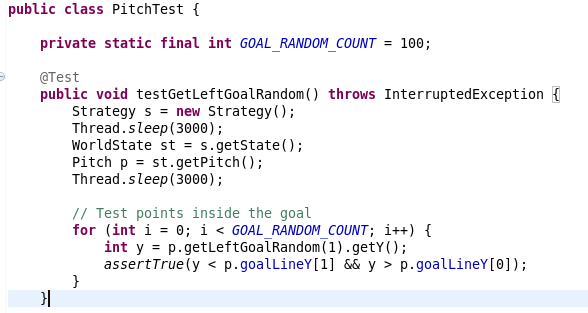
\includegraphics[width=130mm]{test-example.png}
\end{figure}

\subsection{Figure 2: Ball Prediction working, showing reflection}

\begin{figure}[ht!]
\centering
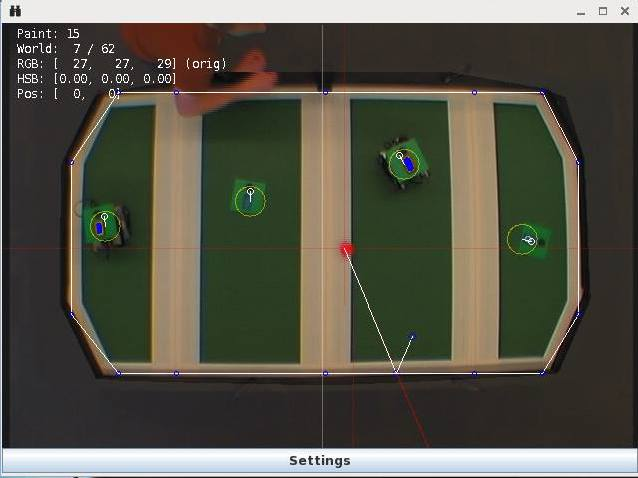
\includegraphics[width=130mm]{system2.jpg}
\end{figure}

\subsection{Figure 3: Example of a tutorial on our wiki}

\begin{figure}[ht!]
\centering
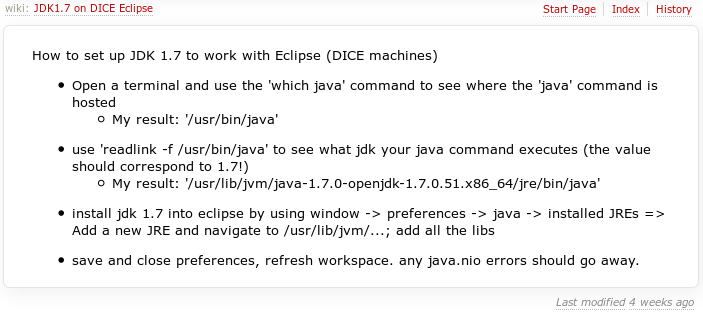
\includegraphics[width=160mm]{tutorial-example.png}
\end{figure}

\subsection{Figure 4: Abstract Robot method: goToFast()}

\begin{figure}[ht!]
\centering
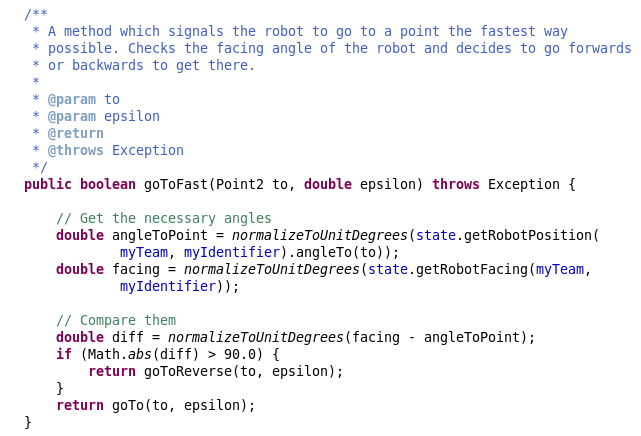
\includegraphics[width=130mm]{strategy-example.png}
\end{figure}

\end{document}



